% !TEX program = xelatex
% !TEX options = --shell-escape 
\documentclass[12pt,AutoFakeBold,a4paper]{article}
\usepackage[utf8]{inputenc}
%\usepackage[UTF8]{ctex}
\usepackage[T1]{fontenc}
\usepackage{amsmath}
\usepackage{amsfonts}
\usepackage{amssymb}
\usepackage{makeidx}
\usepackage{ulem} 
\usepackage{graphicx}
\usepackage{ctex}
\usepackage{ulem}

\usepackage{mdframed}
\usepackage[cache=false]{minted}
% 代码插入采用minted,编译时需要开启-shell-escape设置,如无需要可以注释掉相关内容
\usepackage{hyperref}
\let\olditemize=\itemize \let\endolditemize=\enditemize \renewenvironment{itemize}{\olditemize \itemsep0em}{\endolditemize}

\let\oldenumerate=\enumerate \let\endoldenumerate=\endenumerate \renewenvironment{enumerate}{\oldenumerate \itemsep0em}{\endoldenumerate}


\usepackage{setspace}
\onehalfspace
%\doublespace
\renewcommand{\ULthickness}{0.8pt}
\renewcommand{\ULdepth}{2pt}
\usepackage[left=3.17cm, right=3.17cm, top=2.54cm, bottom=2.54cm]{geometry}
\usepackage{titlesec}
\titleformat*{\section}{\heiti\zihao{-3}}
\titleformat*{\subsection}{\heiti\zihao{4}}
\titleformat*{\subsubsection}{\heiti\zihao{-4}}

\begin{document}
\begin{center}
		{\heiti\zihao{2} {\bfseries 北\ 京\ 林\ 业\ 大\ 学} }\\[15pt]
		{\heiti\zihao{3} {\bfseries \underline{2019}学年— \underline{2020}学年第 \underline{2}学期\underline{  数据挖掘  }实验报告书 }}
	\end{center}
	\heiti\zihao{-3}
	\begin{center}
		\makebox[2.5cm][l]{专\hspace{2em}业:}\underbar{\makebox[3.5cm][c]{ 计算机创新}}\hspace*{2cm}\makebox[2.5cm][l]{班\hspace{2em}级:}\underbar{\makebox[3.5cm][c]{计创17班}}
	\end{center}
	\begin{center}
		\makebox[2.5cm][l]{姓\hspace{2em}名:}\underbar{\makebox[3.5cm][c]{窦勇强 }}\hspace*{2cm}\makebox[2.5cm][l]{学\hspace{2em}号:}\underbar{\makebox[3.5cm][c]{171001209}}
	\end{center}
	\begin{center}
	\makebox[2.5cm][l]{实验地点:}\underbar{\makebox[3.5cm][c]{计算中心}}\hspace*{2cm}\makebox[2.5cm][l]{任课教师:}\underbar{\makebox[3.5cm][c]{王建新}}
\end{center}
\begin{center}
	\makebox[3cm][l]{实验题目:}\underbar{\makebox[11cm][c]{马尔科夫模型和隐马尔科夫模型}}
\end{center}
\begin{center}
	\makebox[3cm][l]{实验环境:}\underbar{\makebox[11cm][c]{Python 3.7, PyCharm by JetBrain
}}
\end{center}

%\noindent 实验要求:
%
%\vspace{0.5em}\noindent 实验内容:
%
%\vspace{0.5em}\noindent 实现方法、实验结果及结论分析等:
\songti \zihao{-3}
\section{实验要求}
\begin{enumerate}
%\setlength\itemsep{1em}
\item 掌握马尔科夫模型和隐马尔科夫模型的原理和算法。
\item 能够利用模型编写相应的程序。
\item 能够利用编写的程序解决实际问题,包括训练模型参数、识别和预测。
\end{enumerate}

\section{实验内容}
\subsection{实验背景介绍}
马尔可夫模型和隐马尔科夫模型不仅仅广泛应用于语音识别和自然语言理解。下面就是一个例子:

中国湖南湖北一带有一句歇后语“下雨天打孩子——闲着也是闲着”。其实“打孩子”是谐音,实际上是“打鞋子”,也就是制作草鞋的意思。表达的大致意思是:下雨天不能出去到地里劳作,就在家利用空闲的时间预备一些草鞋。一段时间的观察结果如下:
\begin{figure}[H]
\centering
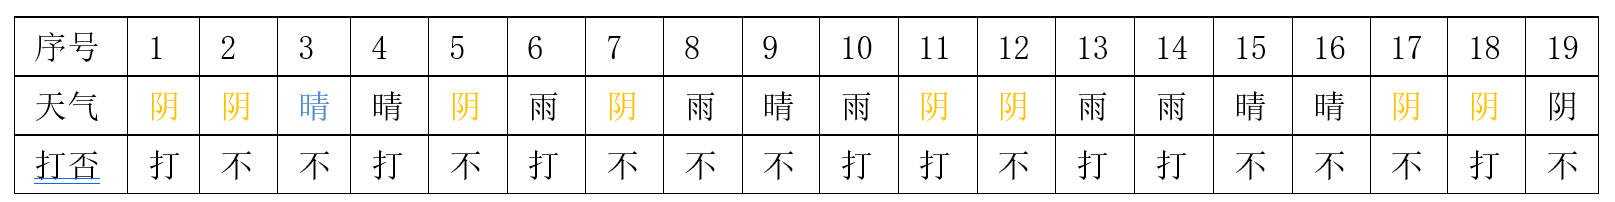
\includegraphics[scale=0.8]{figures/pic1.png}

\caption{一段时间的观察结果}
\label{fig:pic1}
\end{figure}
如果天气情况看作状态,打孩子/不打孩子看作观察结果,那么这是一个典型的隐马尔科夫模型系统。根据上表数据,推算状态转移矩阵A(是一个3乘3的矩阵),和状态到观察值的条件概率矩阵(是一个3乘2的矩阵)。状态的初始概率暂时用整体的概率来表示。
如果今天阴天,请计算后天“打孩子”的概率。

有了初步的三种值:初始状态概率、状态转移矩阵和状态到观察值的条件概率,那么在知道一串观察值“打”与“不打”的情况下,要进行模型推断:包括初始状态概率值(是一个向量)、状态转移概率(是一个方阵)、状态到观察值之间的概率(一个矩阵)。

\subsection{输入输出及具体要求}
首先,关于训练模型:

输入:一个或多个观察值序列,是一个或多个“打-不”串,分别表示(“打”和“不打”)。

输出:通过模型迭代计算,得到状态初始概率值向量、状态转移方阵、状态到观察值之间的概率矩阵。
\newline

第二,关于概率计算(在已经获取模型的基础上):

输入:一个“打-不”串,分别表示(“打”和“不打”)。

输出:该串出现的概率。
\newline

第三,关于识别(在已经获取模型的基础上):

输入:一个观察值序列,是一个“打-不”串,分别表示(“打”和“不打”)。

输出:观察值背后的状态序列,字符串用三个字符“晴”、“阴”、“雨”表示。

\section{实现方法}
本次实验依旧在之前实验编写的dmarsenal的Python package包内迭代开发。

关于HMM模型的训练采用Baum-Welch算法,即EM算法

关于模型给定观测序列预测状态(类似于语音识别)的实现采用Viterbi算法,即动态规划算法。


下面列出的是几个实现的核心部分,便于在报告中查看。
\subsection{图片插入示例}
\begin{figure}[H]
\centering
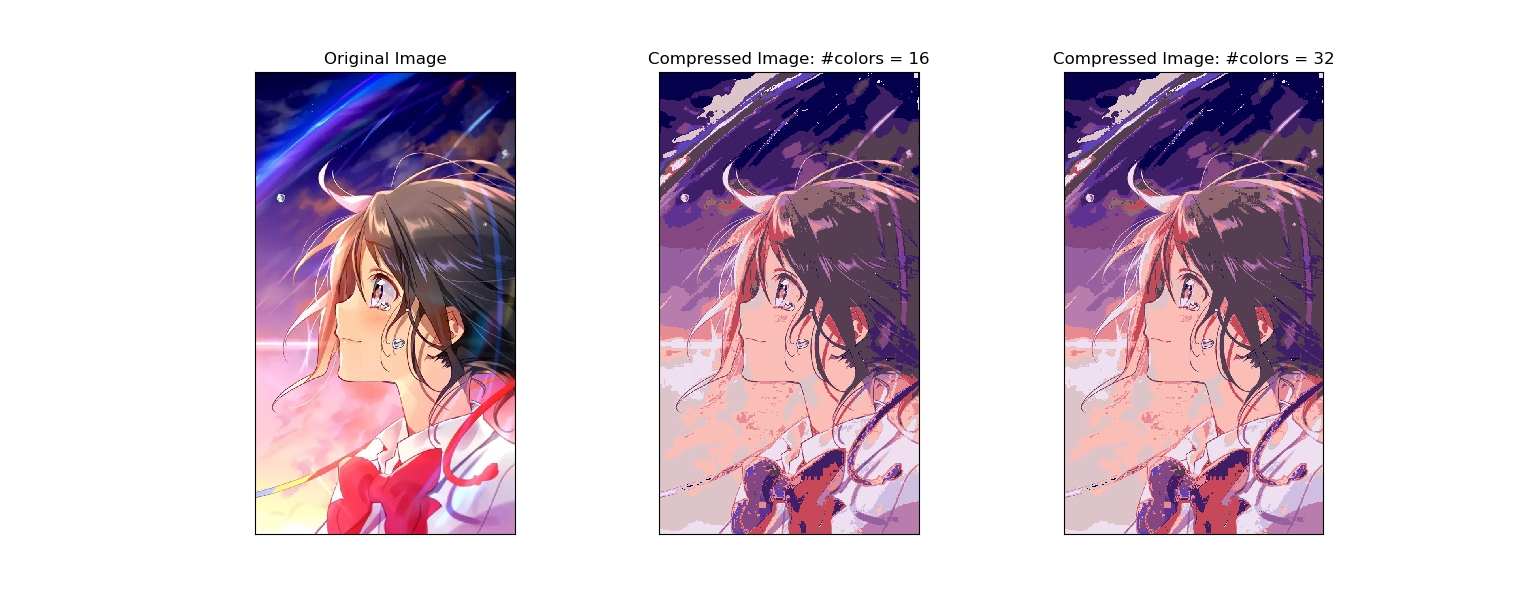
\includegraphics[width=\textwidth]{figures/image_compression_human.png}

\caption{聚类图像压缩测试}
\label{fig:cluster}
\end{figure}


\subsection{代码片段示例}
\inputminted[linenos,
			frame=lines,
			baselinestretch=1,
%			bgcolor=LightGray,
			fontsize=\small
			 ]{python}{code/hmm_demo.py}

\subsection{数据预处理}
如上面的代码所示,实现了状态序列内部表示序号,以及序号到状态等的数据序列转换。
 
\section{实验结果}
\subsection{模型的训练、概率计算及预测}
大概经过55次迭代后,模型对于观测序列的预测概率收敛至4.285618182223047e-05,具体如下图所示。
\begin{figure}[H]
\centering
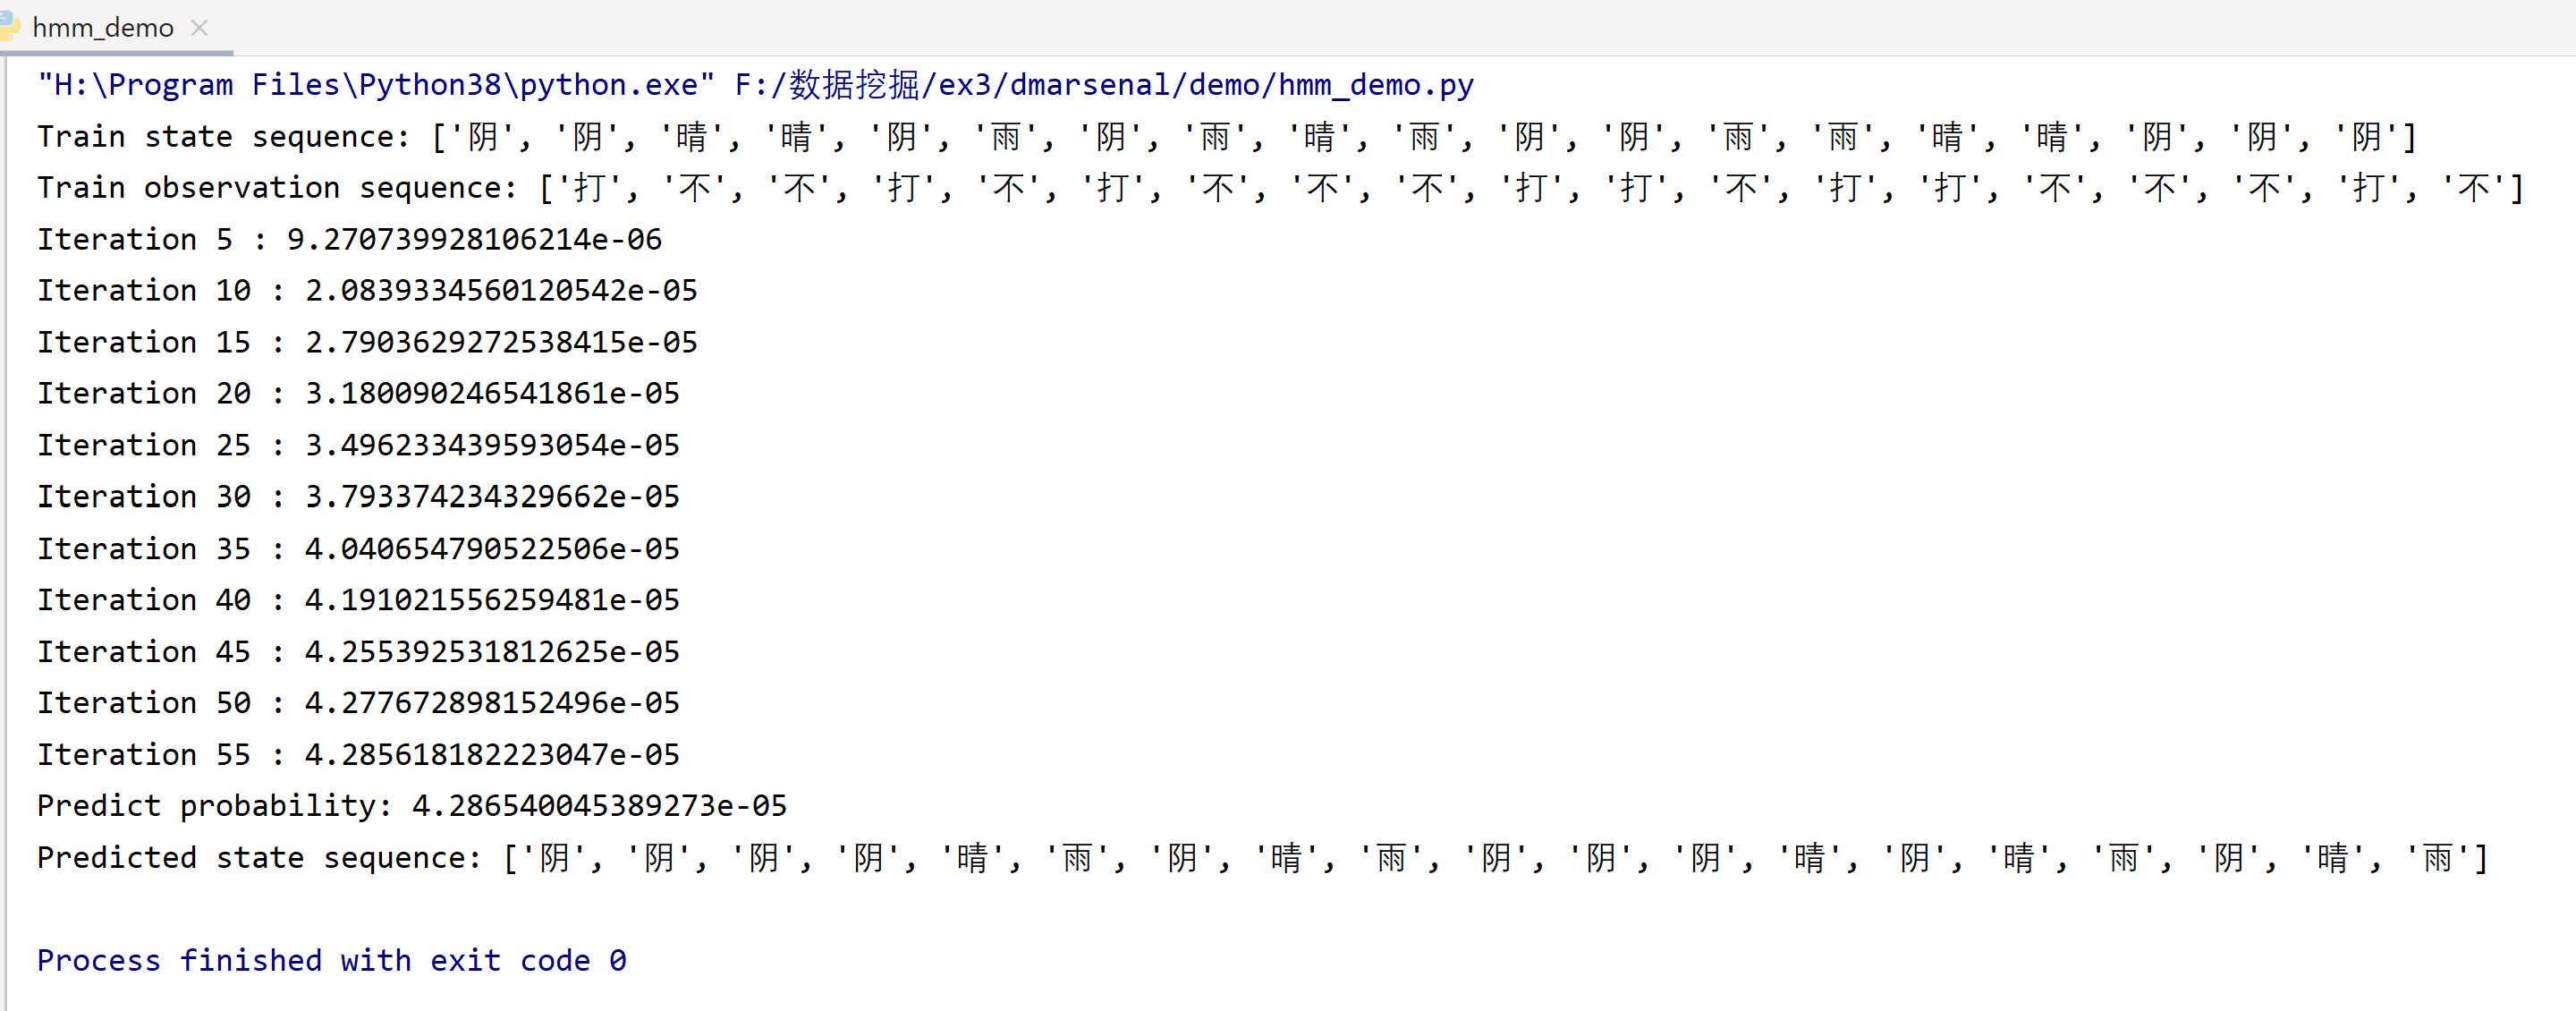
\includegraphics[width=0.9\textwidth]{figures/hmm_output.png}
\caption{HMM模型的训练、概率计算及预测结果}
\label{fig:out}
\end{figure}
\subsection{模型数据预测结果}
原始序列的状态:

['阴', '阴', '晴', '晴', '阴', '雨', '阴', '雨', '晴', '雨', '阴', '阴', '雨', '雨', '晴', '晴', '阴', '阴', '阴']
\newline

训练好模型的预测状态结果:

['阴', '阴', '阴', '阴', '晴', '雨', '阴', '晴', '雨', '阴', '阴', '阴', '晴', '阴', '晴', '雨', '阴', '晴', '雨']

\section{心得体会}
\begin{enumerate}

\item Viterbi算法类似于多段图的最短路径问题,通过动态规划的思想求解出达到最优概率值隐藏状态序列。

\item Baum-Welch算法(EM算法)可以在无监督的情况下,同时不知道状态序列和模型参数来进行E步和M步的迭代求解。并且初始的模型参数不会对于结果造成较大影响,最终都会收敛到一个比较好的概率值

\item 书上的是关于有一个观测序列去训练HMM模型,当有多个观测序列的时候,在独立性假设下,整个的似然值等于每个序列的概率值的乘积,只需要在EM算法更新参数时进行修改为多个序列就好。参考: 

\href{https://www.zhihu.com/question/383437650/answer/1153730978}{https://www.zhihu.com/question/383437650/answer/1153730978},\href{https://www.zhihu.com/question/49189633}{https://www.zhihu.com/question/49189633}

\item 关于在无监督学习的Baum-Welch算法不需要标签去训练和预测的时候隐藏状态的对应问题需要进一步学习和研究。

 
\end{enumerate}

\end{document}
